\documentclass[tikz,border=3pt]{standalone}
\usepackage{amsmath,bm,xcolor}
\usetikzlibrary{arrows.meta}
\begin{document}
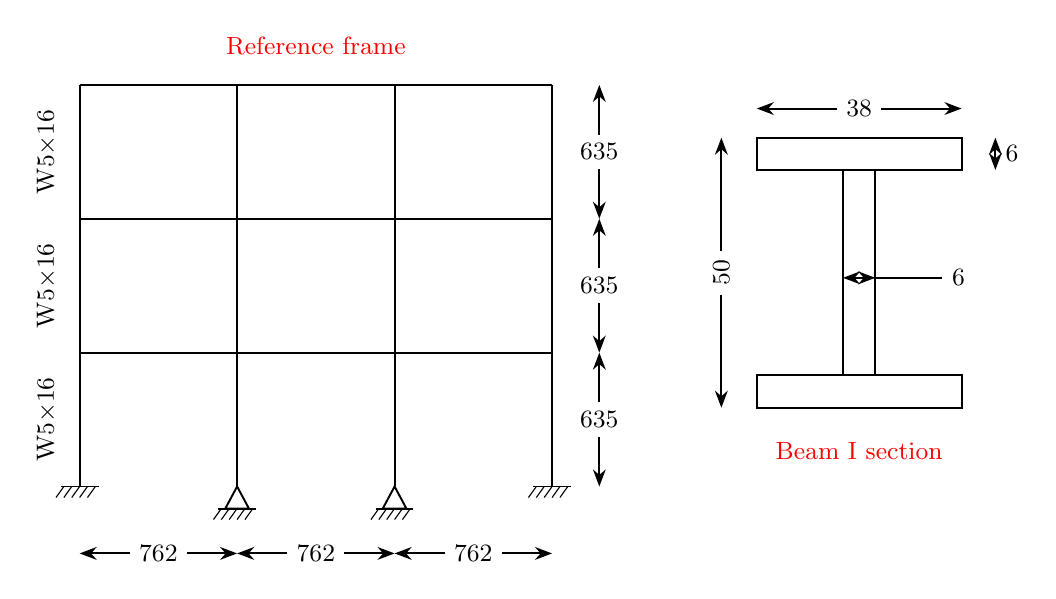
\begin{tikzpicture}[>=Stealth,every node/.style={font=\fontsize{9}{11}\selectfont},line width=.7pt]
\draw[] (0,0)--(0,5.1);
\draw[black] (-0.24,0)--(0.24,0);
\draw[black,line width=.4pt] (-0.2,0)--(-0.3,-0.14);
\draw[black,line width=.4pt] (-0.1,0)--(-0.2,-0.14);
\draw[black,line width=.4pt] (0,0)--(-0.1,-0.14);
\draw[black,line width=.4pt] (0.1,0)--(0,-0.14);
\draw[black,line width=.4pt] (0.2,0)--(0.1,-0.14);
\draw[] (2,0)--(2,5.1);
\draw[black] (2,0)--(1.85,-0.28)--(2.15,-0.28)--cycle;
\draw[black] (1.76,-0.28)--(2.24,-0.28);
\draw[black,line width=.4pt] (1.8,-0.28)--(1.7,-0.42);
\draw[black,line width=.4pt] (1.9,-0.28)--(1.8,-0.42);
\draw[black,line width=.4pt] (2,-0.28)--(1.9,-0.42);
\draw[black,line width=.4pt] (2.1,-0.28)--(2,-0.42);
\draw[black,line width=.4pt] (2.2,-0.28)--(2.1,-0.42);
\draw[] (4,0)--(4,5.1);
\draw[black] (4,0)--(3.85,-0.28)--(4.15,-0.28)--cycle;
\draw[black] (3.76,-0.28)--(4.24,-0.28);
\draw[black,line width=.4pt] (3.8,-0.28)--(3.7,-0.42);
\draw[black,line width=.4pt] (3.9,-0.28)--(3.8,-0.42);
\draw[black,line width=.4pt] (4,-0.28)--(3.9,-0.42);
\draw[black,line width=.4pt] (4.1,-0.28)--(4,-0.42);
\draw[black,line width=.4pt] (4.2,-0.28)--(4.1,-0.42);
\draw[] (6,0)--(6,5.1);
\draw[black] (5.76,0)--(6.24,0);
\draw[black,line width=.4pt] (5.8,0)--(5.7,-0.14);
\draw[black,line width=.4pt] (5.9,0)--(5.8,-0.14);
\draw[black,line width=.4pt] (6,0)--(5.9,-0.14);
\draw[black,line width=.4pt] (6.1,0)--(6,-0.14);
\draw[black,line width=.4pt] (6.2,0)--(6.1,-0.14);
\draw[] (0,1.7)--(6,1.7);
\draw[] (0,3.4)--(6,3.4);
\draw[] (0,5.1)--(6,5.1);
\draw[<->] (0,-.85)--(2,-.85) node[midway,fill=white] {762};
\draw[<->] (2,-.85)--(4,-.85) node[midway,fill=white] {762};
\draw[<->] (4,-.85)--(6,-.85) node[midway,fill=white] {762};
\draw[<->] (6.6,0)--(6.6,1.7) node[midway,fill=white] {635};
\draw[<->] (6.6,1.7)--(6.6,3.4) node[midway,fill=white] {635};
\draw[<->] (6.6,3.4)--(6.6,5.1) node[midway,fill=white] {635};
\node[rotate=90] at (-0.42,0.85) {W5$\times$16};
\node[rotate=90] at (-0.42,2.55) {W5$\times$16};
\node[rotate=90] at (-0.42,4.25) {W5$\times$16};
\node[red] at (3,5.6) {Reference frame};
\begin{scope}[shift={(8.6,1.0)}]
\draw (0,0) rectangle (2.6,.41);
\draw (0,3.02) rectangle (2.6,3.43);
\draw (1.095,.41) rectangle (1.505,3.02);
\draw[<->] (0,3.8)--(2.6,3.8) node[midway,fill=white] {38};
\draw[<->] (-.45,0)--(-.45,3.43) node[midway,fill=white,rotate=90] {50};
\draw[<->] (3.03,3.02)--(3.03,3.43) node[midway,right] {6};
\draw[<->] (1.095,1.65)--(1.505,1.65);
\draw (1.505,1.65)--(2.35,1.65) node[right] {6};
\node[red] at (1.3,-.55) {Beam I section};
\end{scope}

\end{tikzpicture}
\end{document}
